\chapter{Informationsbeschaffung}
\label{chap:Informationsbeschaffung}
Dieses Kapitel bietet fundamentale physikalische Gegebenheiten, sowie die relevanten Eigenheiten des verwendeten \ac{PIR}-Sensors. Da es sich um eine bildgebendes Messprinzip handelt, werden des Weiteren geometrische Aspekte erläutert. Schlussendlich bietet dieses Kapitel auch nötige Informationen über das Messobjekt bzw. die Messumgebung geliefert.

\section{Grid-Eye AMG8834}
\label{sec:AMG8834}

Der verwendete Panasonic AMG8834 ist ein bildgebender \ac{MEMS}-Sensor, der mit insgesamt 64 temperaturempfindlichen Thermosäulenelementen ausgestattet ist. Diese sind als 8x8 Pixel-Matrix auf den Chip aufgebracht. In Abbildung \ref{fig:Explosionsdarstellung} ist der Aufbau des Sensors dargestellt.
 
\begin{figure}[H]
	\centering
	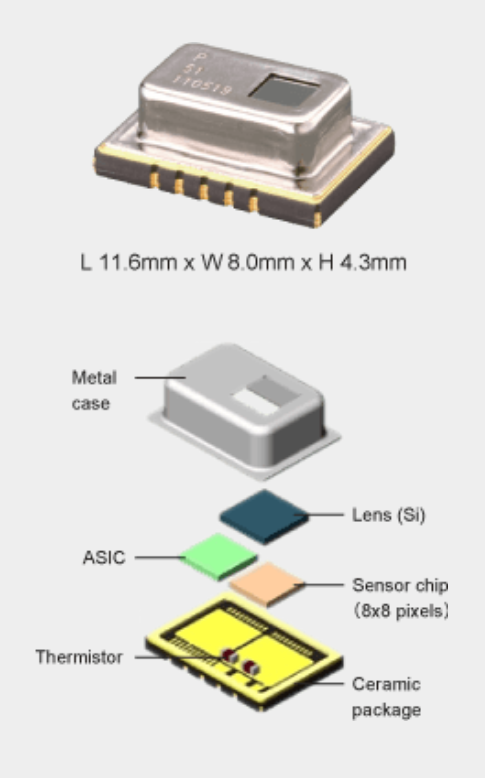
\includegraphics[width=0.3\textwidth]
	{fig/grid_eye_aufbau.PNG}
	\caption[Schema des AMG8834 Sensors]{Schema des AMG8834 Sensors} \protect\cite{AMG8834}
	\label{fig:Explosionsdarstellung}
\end{figure}
Die eintreffenden Infrarotwellen werden durch die Siliziumlinse, welche einen \ac{FOV} von 60$^\circ$ besitzt, gefiltert. Dabei durchdringen lediglich langwellige Infrarotstrahlungen mit den Wellenlängen 8-13 $\mu$m die Linse. Dies entspricht dem dritten atmosphärischen Fenster.

In Abbildung \ref{fig:SchemaAMG8834} ist das Prinzipschema des Sensors darstellt. Das Messprinzip des Sensors wird im Unterkapitel \ref{subsec:seebeck} detailliert erläutert. Die entstandene Thermospannung wird durch die \ac{ASIC} des \ac{MEMS}-Sensor verarbeitet. Das selektierte Thermospannung wird verstärkt, mit dem integrierten Thermistor verglichen und mit dem \ac{ADC} gewandelt. Durch die hohe interne Verstärkung besitzt der Sensor jedoch bei normalen Bedingungen\footnote[2]{Umgebungstemperatur 0-80 $^\circ$C bei Luftfeuchtigkeit 15-85\%} eine Genauigkeit von +/- 3°C. 

\begin{figure}[H]
	\centering
	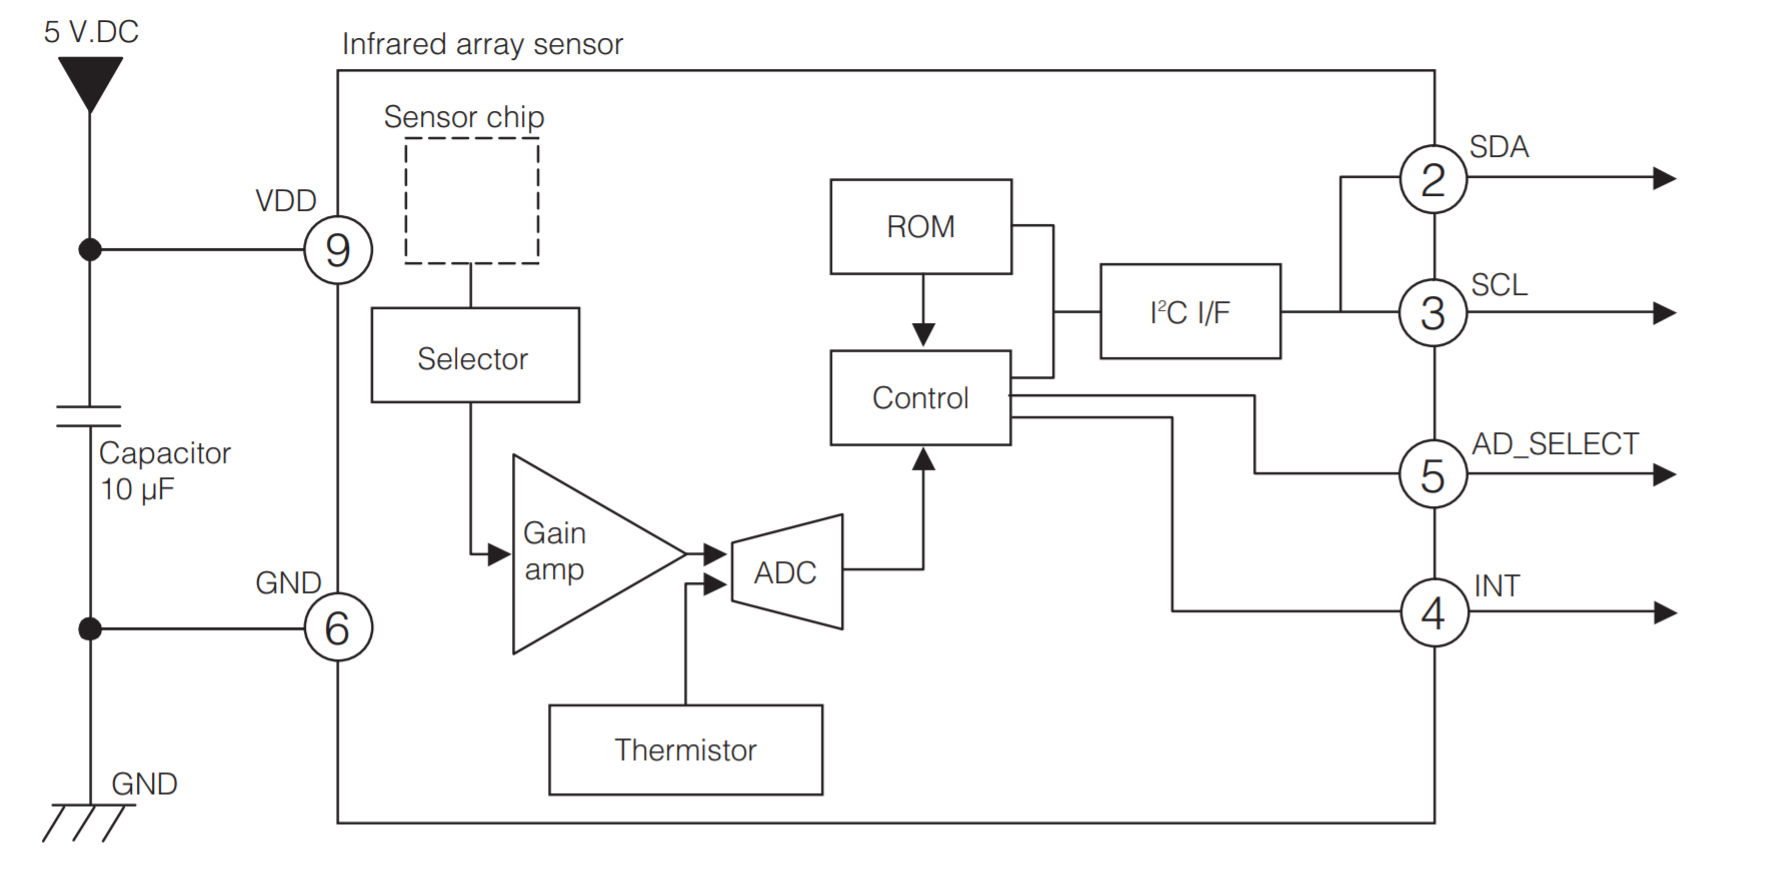
\includegraphics[width=0.75\textwidth]
	{fig/Circuit_AMG8834.PNG}
	\caption[Schema des AMG8834 Sensors]{Schema des AMG8834 Sensors} \protect\cite{AMG8834}
	\label{fig:SchemaAMG8834}
\end{figure}
 
Über die \ac{I2C} lassen sich die Werte der Thermoelemente und der Thermistoren je aus 2 Register auslesen. Die Messwerte werden alle 100 ms aktualisiert. Dabei werden lediglich 12 Bit pro Pixel für die Temperaturregister genutzt. Dies führt zu der kleinsten unterscheidbaren Größe von 0.25 $^\circ$C . Die Thermistorregister lassen sich mit der Auflösung von 0.625 $^\circ$C unterscheiden. In Abbildung \ref{fig:SchemaAMG8834} ist klar ersichtlich, dass die Umgebungstemperatur, bzw. die Temperatur, welche vom Thermistor gemessen wird direkten Einfluss auf die Pixelwerte besitzen. Variieren die Thermistorwerte aufgrund von Raumtemperaturschwankungen können die Pixelwerte dadurch bedeutende Abweichungen entstehen.

\section{Physikalische Aspekte}
\label{sec:Physik}
Dieser Abschnitt erläutert auf kurze und prägnante Weise, physikalischen Aspekte die dem Sensor zu Grunde liegen. Dies bietet die Grundlage für die Bestimmung der Störquellen und das Verhalten des Sensors bei entsprechenden äußeren Einwirkungen. Die Tabelle \ref{tab:Legende Physikalische Grössen} gibt die Bezeichnungen der nachfolgenden Formeln wieder.

\begin{table}[H]
	\centering
	\begin{tabular}{l|c|c}
		\rowcolor{gray} Grösse &  Bezeichnung  & Einheit \\
		\hline 
		Thermospannung &  $ U_{t}$ & $J$  \\ 
		\rowcolor{gray} Thermokraft P/N -Silizium  & $\alpha_{p},\alpha_{n}$ & $V/K$\\	
		Temperatur P/N -Silizium &  $T_{p},T_{n}$ & $V/K$ \\
		\rowcolor{gray}Wärmestrom &  $\dot{Q}$ & $J$  \\ 
		Emission & $\epsilon$ & $-$\\	
		\rowcolor{gray}Reflektion &  $\rho $ & $-$ \\
		Transmission & $\tau$ & $-$\\
		\rowcolor{gray}Absoprtion &  $\alpha$ & $-$  \\ 
		Strahlungsleistung & $\dot{Q}$ & $W$\\
		\rowcolor{gray}spektrale spezifische Ausstrahlung &  $M_{\lambda }$ & $W/sr$\footnote[3]{Steradiant: Messeinheit für den Raumwinkel} \\
		Planksches Wirkungsquantum &  $ h$ & Js \\ 
		\rowcolor{gray} Lichtgeschwindigkeit im Vakuum & $c $ & $ m/s$ \\ 
 		Stefan-Boltzmann-Konstante & $\sigma$ & $ W/m^2K^2 $ \\ 
	\end{tabular}
	\caption{Legende physikalische Grössen Konzeptzeichnungen}
	\label{tab:Legende Physikalische Grössen} 
\end{table} 


\subsection{Seebeck-Effekt}
\label{subsec:seebeck}
Die durch die konvexe Linse gesammelten Infrarotstrahlen verursachen auf den einzelnen Thermosäulenelemente (2), dass die Oberfläche erwärmt wird. Es entsteht zwischen der erwärmten, n-dotierten Siliziumschicht (4) und der kühleren p-dotierten Siliziumschicht (6) ein Temperaturgefälle.   

\begin{figure}[H]
	\centering
	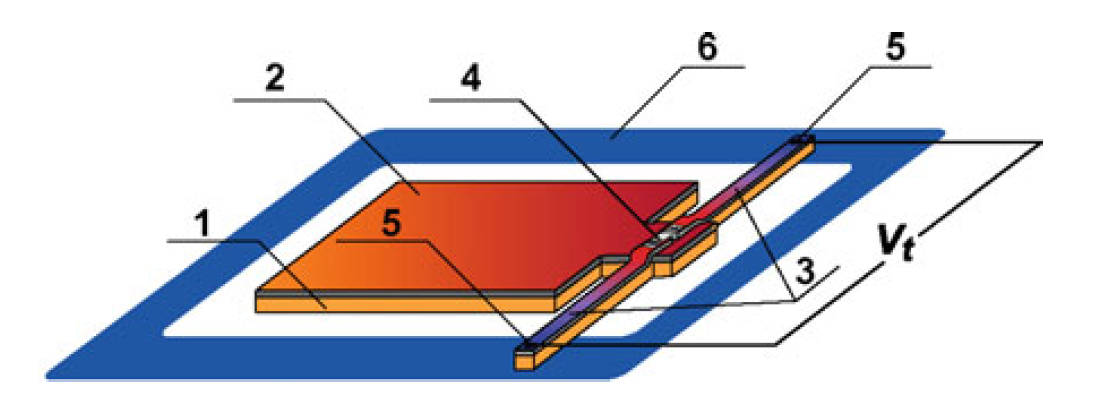
\includegraphics[width=0.6\textwidth]
	{fig/Mems_Thermopile.PNG}
	\caption[Aufbau Thermosäulenelement]{Aufbau Thermosäule} \protect\cite{AMG8834}
	\label{fig:AufbauThermo}
\end{figure}

\todo{Kotrolle Thermosäule} Durch die unterschiedlichen Thermokräfte (auch Seebeckkoeffizienten) der zwei Halbleitermaterialien entsteht ein Potentialunterschied, den man an den Punkten 3 und 5 abgreifen kann. Diese Spannung $U_{t}$ ist die Grundlage des Messprinzips und wird mit Formel \ref{eq1} \protect\cite{AMG8834} beschrieben.


\begin{equation}
\label{eq1}
U_{t} = (\alpha_{p} + \alpha_{n})*(T_{p}+T_{n})
\end{equation}
\begin{center}

\end{center}
\myequations{Seebeck-Effekt}


\subsection{Strahlungstheorie}
\label{subsec:Strahlungstheorie}
Das vorherige Unterkapitel erläutert die Funktion des Sensors als Infrarotempfänger. Nicht unwesentlich ist weiter die Betrachtung des Senders. Grundsätzlich gilt, jeder Körper, der eine Temperatur oberhalb des absoluten Nullpunkt aufweist, strahlt Wärmestrahlung im Infrarotbereich ab. 

Im Allgemein wird für die Betrachtung vom Plank'schen Strahlungsgesetz ausgegangen. Nach dieser gilt für eine spektrale spezifische Ausstrahlung eines Schwarzkörpers mit der Temperatur T folgende Formel \protect\cite{Thermoformeln}:

\begin{equation}
\label{eq2}
M_{\lambda } = \frac{2\pi h c^2 }{\lambda^5}*\frac{1}{e^\frac{hc}{\lambda k_{B} T}-1}
\end{equation}
\myequations{Plank'sches Strahlungsgesetz}

Wie in der Formel ersichtlich ist die Ausstrahlung eines schwarzen Körper mit 5. Potenz von der Wellenlänge und exponentiell von der Temperatur abhängig. Durch die Siliziumlinse des Sensors werden somit Störquellen, welche andere Wellenlängen aufweisen, gefiltert. Dies ist vor allem bei Lichtquellen ein relevante Eigenschaft.

Das Stefan-Boltzmann-Gesetz \protect\cite{Thermoformeln} gibt die Strahlungsintensität $\dot{Q}$ eines idealen Temperaturstrahlers an. Diese Formel bietet für die Anwendung die relevantesten Erkenntnisse.


\begin{equation}
\label{eq3}
\dot{Q} = \frac{\mathrm{d} Q}{\mathrm{d} t} = \epsilon *\sigma * A * T_{obj}^4
\end{equation}
\myequations{Wärmestrahlung }

\begin{figure}[H]
	\centering
	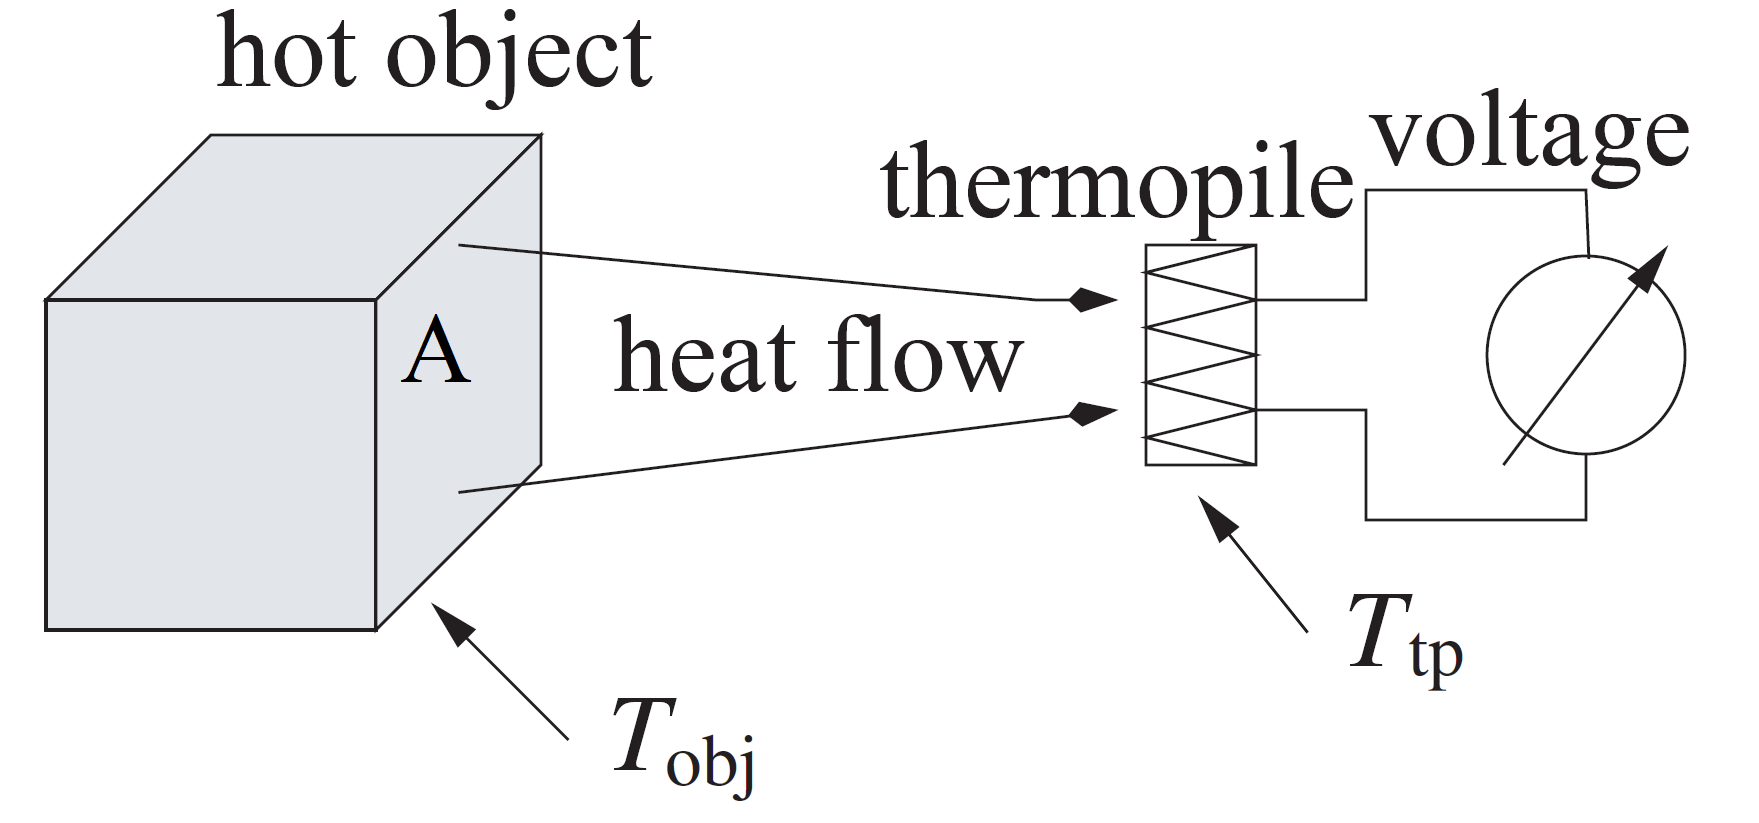
\includegraphics[width=0.5\textwidth]
	{fig/seebeck2.PNG}
	\caption[Aufbau Thermosäule]{Aufbau Thermosäule} \protect\cite{seebeck}
	\label{fig:thermosäule}
\end{figure}

Diese Formel zeigt auf, dass die Wärmestrahlung eines Körpers im wesentlichsten (mit 4. Potenz)
von der eigenen Temperatur abhängig ist. Die Fläche A ist lediglich proportional. Dies verursacht, dass bereits flächenmäßig kleine, jedoch stark erwärmte Objekte im Messbereich einen bedeutenden Einfluss auf die Messresultate liefern können. Zusätzlich Verursachen Wärmequellen im nahen Umfeld des Messbereichs Abweichungen auf die Messresultate.

Des Weiteren weist diese Formel auf eine weitere Problematik dieses Messprinzips hin, der mit dem Emissionsgrad $\epsilon$  in Verbindung steht. Der Emissionsgrad $\epsilon$ ist ein materialabhängiger, jedoch wellenlängenunabhängier Faktor, welcher zwischen 0-1 angegeben wird. Dieser gilt für graue Körper d.h. für Körper, dessen Oberfläche auftreffende Strahlung nicht vollständig absorbieren. Diese Eigenheit gilt für alle realen Körper. 

Nach dem Energieerhaltungsgesetz \protect\cite{Thermoformeln} gilt für Transmission, Reflexion und Absorption die Formel \ref{eq4}.
\begin{equation}
\label{eq4}
\tau  + \alpha + \varphi  = 1
\end{equation}
\myequations{Schwarzer Stahler, Energieerhaltung}

Wobei bei thermischen Gleichgewicht angenommen werden kann, dass der Emissionsgrad der Absortion entpsricht.

\begin{equation}
\label{eq5}
\epsilon \approx  \alpha
\end{equation}
\myequations{Strahlung Energieerhaltung Festkörper}


Da es sich Aufzügen nur von Festkörper ausgegangen wird, fällt die Transmission $\tau$ aus der Gleichung. Es können lediglich Reflexionen oder die Emission des Körpers Einfluss auf die einwirkende Infrarotstrahlung nehmen. Weitere Betrachtungen diesbezüglich werden im Unterkapitel 2.4. gemach

\section{geometrische Aspekte}
\label{sec:geometrie}

Da die Strahlungsintensität mit zunehmender Distanz mit zweiter Potenz abnimmt, spielt die Distanz zum Messobjekt eine entscheidende Rolle. Ein weiteres Kriterium ist der begrenzten \ac{FOV} des Sensors von 60$^\circ$. In der nachstehenden Skizze (Abbildung \ref{fig:Geometrie}) sind die Verhältnisse perspektivisch dargestellt. Dabei wird von einer Raumhöhe von 2.10 m ausgegangen. (nach Standardkabine EN 81-70)   

\begin{figure}[H]
	\centering
	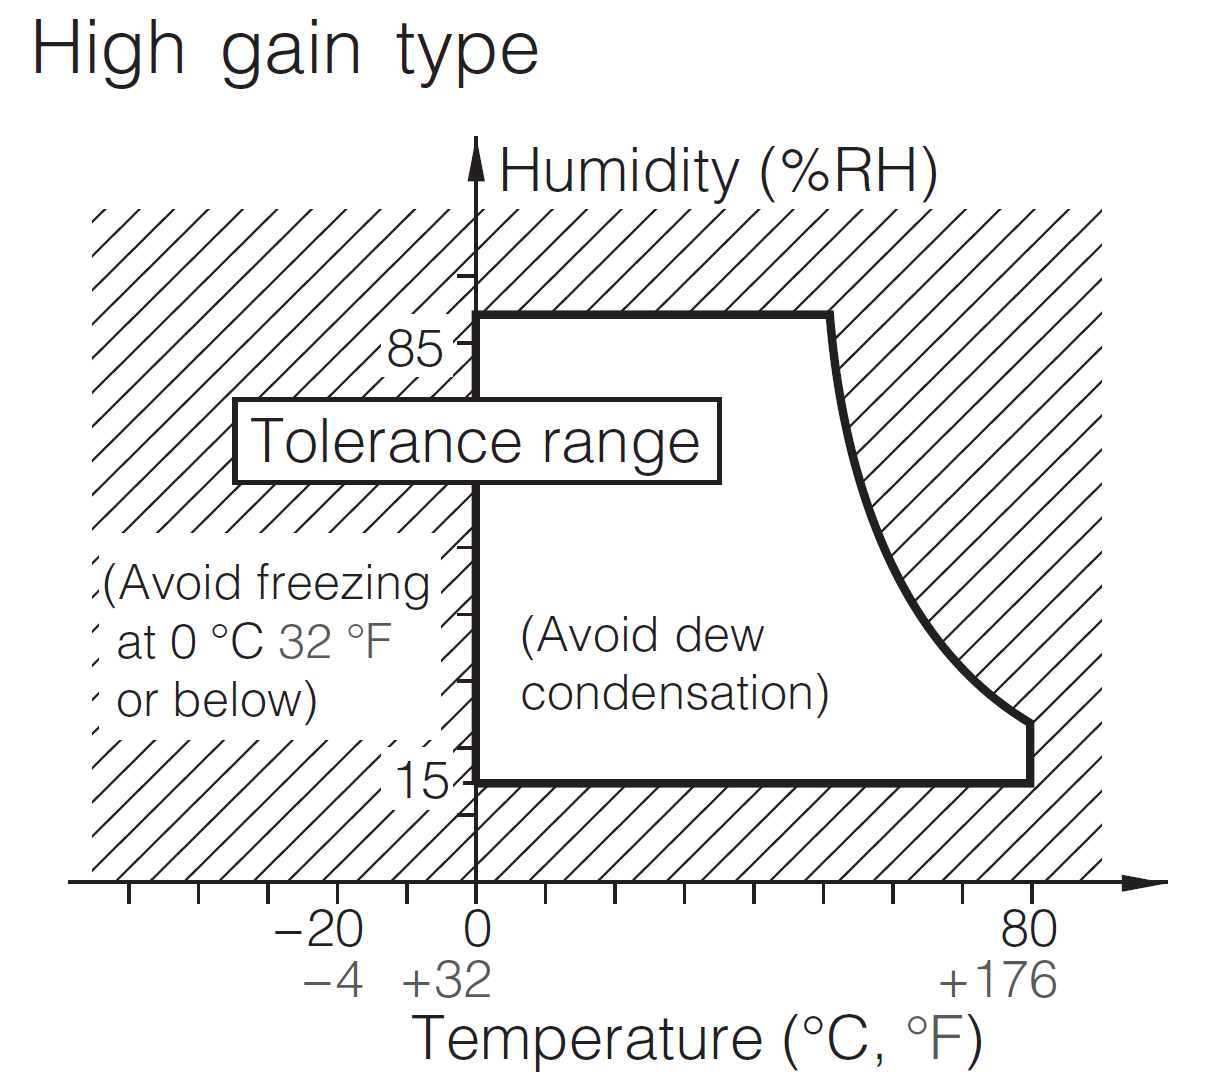
\includegraphics[width=0.5\textwidth]
	{fig/Humidity_Tolerance.PNG}
	\caption[Einfluss Luftfeuchtigkeit]{Einfluss Luftfeuchtigkeit} \protect\cite{AMG8834}
	\label{fig:Geometrie}
\end{figure}

Die räumliche Streckungen verursacht zusätzlich eine perspektivische Verzerrung, welcher in dieser Betrachtung nicht weiter beachtet wird. Zu sehen ist jedoch deutlich, dass bei der Messung von Personen die Messdistanz zwischen 10 bis 110 Zentimeter am relevantesten ist. In diesem Bereich kann jedoch mit dem aktuellen \ac{FOV} im besten Fall eine Fläche von 0.666 $ m/s^2 $ abgedeckt werden. Um eine Aufzugkabine mit 8 Personen\footnote[1]{Masse: (HxBxT) 2100 x 1100 x 1400 [mm]} bei mittlerem Messbereich wird im optimalen Fall ein Öffnungswinkel von 84°x 109°$^\circ$ benötigt. 

Problematisch kann in diesem Zusammenhang die Abschattung des Messbereichs durch grosse Personen sein, welche zentral positioniert sind. 

 

\section{Messobjekt und Messumgebung}
\label{sec:Messobjekt}
Dieses Kapitel beschreibt die Erkenntnisse bei der Betrachtung des Messobjekts und der Messumgebung. Dabei wurden einerseits die Kennwerte von Personen zusammengetragen, sowie die Messumgebung auf Störquellen und Einflussfaktoren begutachtet. Dank der Firma ARLEWO AG konnten unterschiedliche Aufzüge vermessen und bewertet werden. 

\subsection{Personen}
\label{subsec:Personen}

Die Reaktionen im menschlichen Körper sind auf eine Kerntemperatur von 37 °C. Am kältesten ist die Haut, die etwa 4 bis 7 Kelvin (Grad) kälter ist. Die Aufteilung der verschiedenen Arten der Wärmeabgabe beträgt bei einem ruhenden Menschen in einer Umgebung von 20 °C:


\begin{itemize}
	\item  46 \% Strahlung
	\item  33 \% Konvektion\footnote[2]{Konvektion bezeichnet die Wärmeabgabe an
		das umgebende Medium, in der Regel Luft}
	\item  19 \% Schwitzen
	\item   2 \% Atmung.
\end{itemize}

Die Höhe der Wärmeabgabe hängt im wesentlichen von der Schwere der Tätigkeit und von der Größe der Körperfläche ab. Daraus folgt, dass größere Personen mehr Wärme abgeben. Strahlung und Konvektion nehmen mit zunehmender Umgebungstemperatur bis zum Wert null bei 36 °C ab. Hat die Umgebung die Körpertemperatur erreicht, kann folglich durch Strahlung und Konvektion keine Wärme mehr abgeführt werden. In einer Umgebung mit Temperaturen oberhalb 37 °C kann also die Wärme nur noch durch Schwitzen abgeführt werden.\protect\cite{MenschWaerme}

\begin{figure}[H]
		\centering
	\begin{minipage}[b]{0.4\textwidth}
			\centering

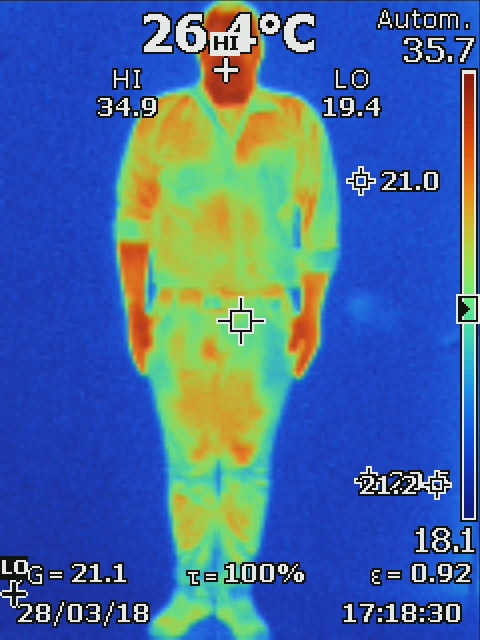
\includegraphics[width=0.8\textwidth]{fig/person_waerme.JPG}
\label{fig:Waermebild}
\caption[Wäermebild eines \\Probanden]{Wärmebild eines \\Probanden}
	\end{minipage}
	\begin{minipage}[b]{0.2\textwidth}
\end{minipage}
	\begin{minipage}[b]{0.4\textwidth}
			\centering
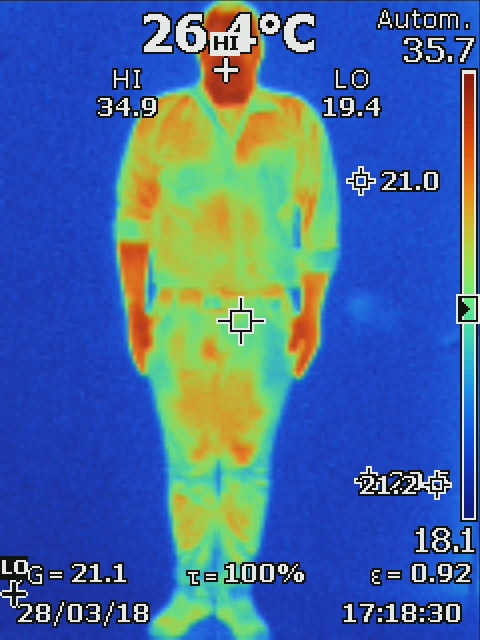
\includegraphics[width=0.8\textwidth]{fig/person_waerme.JPG}
\label{fig:Waermebild2}
\caption[Wäermebild eines \\Probanden]{Wärmebild eines \\Probanden}

	\end{minipage}
	
\end{figure}

Ein weiterer Aspekt, der sehr stark ins Gewicht fällt, ist die Art der Bekleidung. In Abbildung \ref{fig:Waermebild} und Abbildung \ref{fig:Waermebild2} ist deutlich zu sehen, dass das thermische Profil einer Person durch die Bekleidung stark variiert. Bekleidungsfreie Zonen n 

\subsection{Personenaufzüge}

In diesem Unterkapitel wurde der Personenaufzug als Messobjekt näher betrachtet. Neben räumlichen Parametern wie Höhe, Grundfläche und Volumen spielen vor allem die Oberflächenbeschaffenheit bzw. das Oberflächenmaterial Rolle. Weitere thermische Einflussfaktoren finden sich in der Umgebungstemperatur und der verbauten Leuchtmittel.


Wie bereits in \ref{sec:geometrie}

In Abbildung \ref{fig:Edelstahlgewalzt} und \ref{fig:Edelstahlmatt} sind 
\begin{figure}[H]
	\centering
	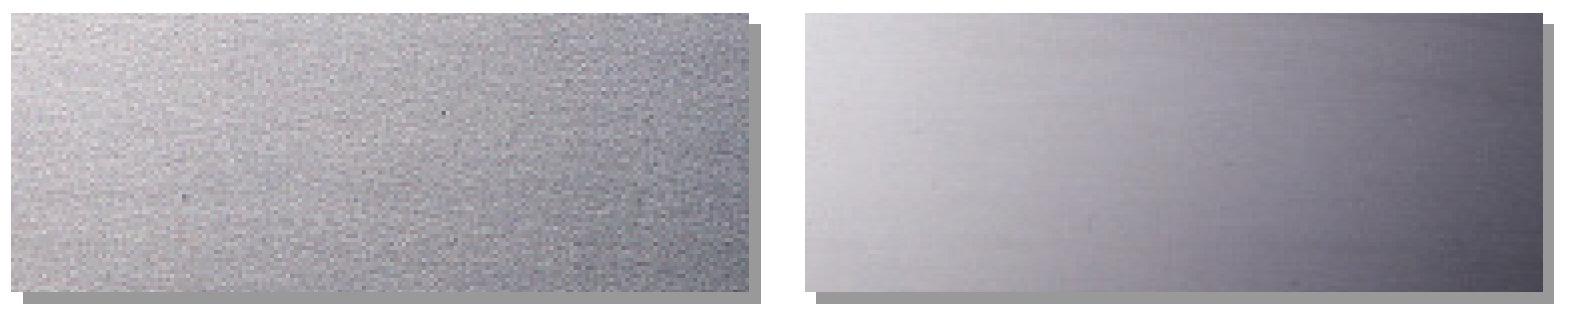
\includegraphics[width=0.8\textwidth]
	{fig/Edelstahl_gewalzt.PNG}
	\caption[Edelstahl warmgewalzt]{Edelstahl warmgewalzt} \protect\cite{Edelstahl}
	\label{fig:Edelstahlgewalzt}
\end{figure}
\begin{figure}[H]
	\centering
	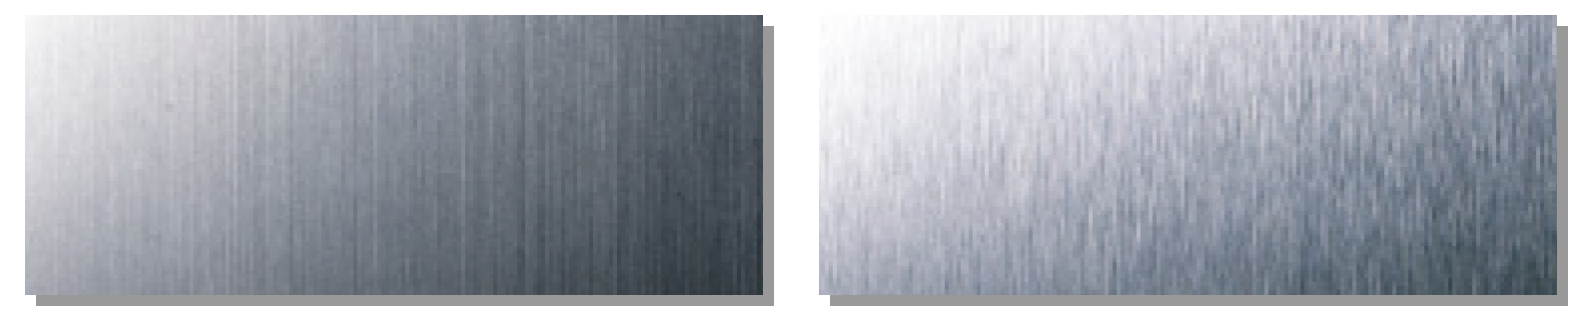
\includegraphics[width=0.8\textwidth]
	{fig/Edelstahl_matt.PNG}
	\caption[Edelstahl kaltgewalzt]{Edelstahl kaltgewalzt} \protect\cite{Edelstahl}
	\label{fig:Edelstahlmatt}	
\end{figure}




\begin{figure}[H]
	\centering
	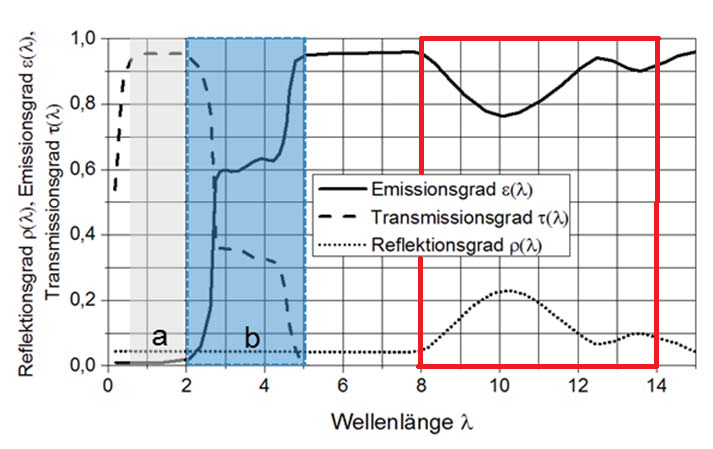
\includegraphics[width=0.8\textwidth]
	{fig/Glas_bearbeitet.png}
	\caption[Emissionsgrad in Abhängikeit zur Wellenlnge]{Emissionsgrad in Abhängikeit zur Wellenlnge} \protect\cite{Edelstahl}
	\label{fig:Glas}	
\end{figure}

\section{Fazit}

Die Personenerkennung in Aufzügen mit \ac{PIR} Sensoren ist am meisten von der Individualität einer Person abhängig. Faktoren wie Körpertemperatur, Körpergröße und Bekleidung verursachen enorme Differenzen. Dadurch kann kein einheitliches Profil erstellt werden. Der geometrische Aspekte Weitere physikalische Gegebenheiten wie die Umgebungstemperatur oder indirekte Sonneneinstrahlung bewirken veränderte Bedingungen für den Messbereich, welche bei einer Messeinheit berücksichtigt werden müssen.     


